\documentclass[../main.tex]{subfiles}

\tikzset
  {phase/.style={draw,minimum width=2.5cm,minimum height=1.5cm,align=center}
  ,previous/.style={below right=0.5cm of #1}
  }
\newcommand\connecttw[2]%
  {\draw[->,thick] (#1) -| (#2);
   \draw[->,thick] (#2) -| (#1);
  }
\newcommand\connectow[2]%
  {\draw[thick, ->] (#1) |- (#2);
  }

\begin{document}
The focus of the chapter is to give the reader an overview of product development methodologies used during the development process of the Thesis problem. The presented methodologies find nowadays vast application in the industry, as they fulfil the  lifelong request of increasing productivity.\\
The chapter is going to analyze Agile and its most famous branch, Scrum. After an introduction of the Agile philosophy, the chapter switch its focus on the Scrum methodology including a comparison with traditional waterfall methods. In the part related to Scrum an overview over tools, processes and roles is given.\\
\section{Agile philosophy}
Agile is presented as a philosophy rather than a methodology. This distinction need to be underlined because its important to understand the direction of the chapter and understand the difference between Agile and Scrum.
The word philosophy is used to emphasize the fact that we are referring to a way of thinking but also on the other hand that we are not trying to give any method to support this way of thinking. Agile set guidelines while Scrum take those guidelines and tells the user exactly 'what to do'.
\begin{figure}
    \centering
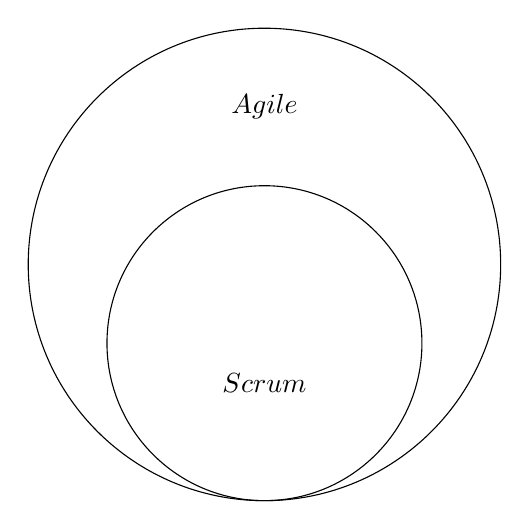
\begin{tikzpicture}
\draw[] (4.5,2) circle[radius = 3];
\node [at={(4.5,4)}] {$Agile$};
\draw [] (4.5,1) circle [radius =2];
\node [at = {(4.5,0.5)}] {$Scrum$};
\end{tikzpicture} 
    \caption{Agile-Scrum relationship}
    \label{fig:SCRUMAGstr}
\end{figure}

\subsection{History of the Agile philosophy}
The definition of a word Agile as a theorized philosophy for product development came only in the early 90´as a result of the Agile Manifesto. It´s important to keep in mind that there where previously approaches that resemble, if not match Agile, those can be inserted under the umbrella term IID, \textit{Iterative Incremental Approaches}.\\
As most of the innovation also the IID ones came from the criticism of previously used methods. In the past most of the methodologies to develop product and in particular to develop software where based on a series of sequential steps which output could only be seen at the end of the process. The series of steps was sometimes so long that the product was already out of the market once completed.\\
The criticism in regard to those methods suggested alternatives approaches which where actually unconsciously filled by Agile ideas such as the response to changes, customer involvement, and working software over documentation.\\
By reading the paper by \citet{larman2003iterative} the traces of iterative and incremental development approaches can be already found in the 30´. \\
Walter Shewahrt, an engineer at Bell Labs, in 1930 posed a series of short "plan-do-study-act" (PSDA) cycles for quality improvement. In those cycles he impemented constant review over results and used this feedback to continue in the development process. This method was a great success and PSDA was vigorously promoted starting from the 40´.\\ 
Tanks to the success the next step for IID was to flood military projects. Iterative approaches were used in the development of the X-15 hyper-sonic jet in which the "Agile like" practices contributed majorly to its success.\\ Post war the IDD experience and experts arrived at NASA, which in the 60´was US government top priority with the ongoing cold war.\\
Project Mercury, the first human spaceflight program of the United States, used short half day iterations. The Development Team performed technical review of all the changes, and applied a super early version of Extreme Programming practice (later theorized Agile-based method) of "test first" development. This consist in writing test before each micro increment. They also applied top-down development with the usage of stubs in the development. A \textit{stub} simulate the behaviour of code or is used as a substitute to yet-to-be-developed code.\\ 
\subsection{Agile Manifesto}
The influences continued until a real theorizing was made in 2001 by software developer that, tired of inefficient way to develop software summed all up under the slogan "\textit{We are uncovering better ways of developing software by doing it and helping others do it}". \\
The proponents of the Manifest found them self in a situation in which no software development methodology or techniques enabled them to succeed in a constant manner. As reported by \citet{schmidt2013software} the Manifesto was to establish a set of principles for software development based on rapid prototyping, incremental product delivery, and absolutely no product design. The Manifesto highlighted 4 values:
\begin{itemize}
    \item Individuals and interactions over processes and tools;
    \item Working software over comprehensive documentation;
    \item Customer collaboration over contract negotiation;
    \item Responding to change over following a plan.
\end{itemize}
Let´s better analyse in details the meaning of each value. 
\subsubsection{Individuals and interactions over processes and tools}
One of Agile goals is to enhance the communications inside teams. The importance of having good interactions between the team members surpass the focus of having high-tech tools or complex processes. \\
The main problem with tools and process is that they push towards a certain conformity. Conformity makes it hard to accommodate new ideas, requirements and way of thinking. Other than that using tools that push towards conformity requires time to "translate" concepts in a tool-understandable way from a team one, indeed consuming time. Agile stays human-centered and team focused. Every member need to be an active participants with its own way of seeing things. 
\subsubsection{Working software over comprehensive documentation}
One of the flaws of waterfall method is related to the fact that a working software version arrives when the initial requirements are already outdated. To criticize this mechanism it´s important to deploy working software as soon as possible during the development process. Having a working product as early as possible is also use full for getting customer feedback on it, as the next values will underline. 
It´s important to state that documentation don´t need to be completely left out but the focus need to be on what brings the most value at a certain time point.
\subsubsection{Customer collaboration over contract negotiation}
This value stresses the importance of encouraging customer and developer team collaboration over the product, other than seeing each other as adversaries in the contract negotiation part.
Creating a strong customer relationship translates into more frequent and accurate customer feedback. The more a customer is involved in the product the more the outcome of a product is shared between developers and the customer itself, thus the push in the direction of success is stronger.  
\subsubsection{Responding to change over following a plan}
This stands as the most innovative values out of the four. The ability not only to respond to changes but to welcome them during the development process is a really important tool for Agile. Differently from other approaches, as for example QFD, in Agile as time and knowledge over the product increases the ability to make changes stay unvaried. This is a really innovative concept. Changes are welcomed and the cost related to implementing changes ideally stay the same until product delivery. In traditional method this cost tend to become bigger as approaching the delivery deadline.
\begin{figure}[H]
\centering
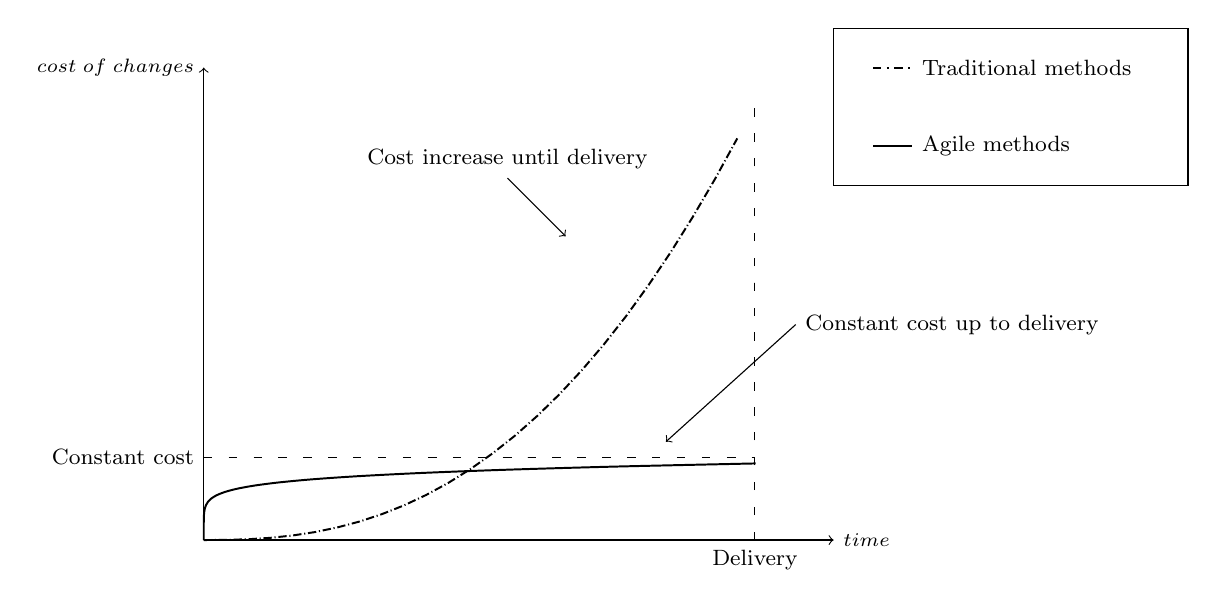
\begin{tikzpicture}
  \draw[->] (0, 0) -- (8, 0) node[right] {\scriptsize $time$};
  \draw[->] (0, 0) -- (0, 6) node[left] {\scriptsize $cost\;of\;changes$};
  \draw[scale=0.7, domain=0:2.42, densely dashdotted, line width=0.25mm, variable=\x, black] plot ({4*\x}, {0.8*\x^2.5});
  \draw[scale=0.7, line width=0.25mm, domain=0:1.39, smooth, variable=\y, black]  plot ({\y^7}, {\y});
  \draw[loosely dashed, scale=0.7, domain=0:10, smooth, variable=\y, black]  plot ({\y}, {1.5});
  \draw[loosely dashed, scale=0.7, domain=0:8, smooth, variable=\x, black]  plot ({10}, {\x});
  \node at (7,0) [align=center,anchor=north ] {\footnotesize Delivery};
  \node at (0,1.05) [align=center,anchor=east ] {\footnotesize Constant cost};
  \draw[<-] (40:6) -- (50:6) node[above] {\footnotesize Cost increase until delivery};
  \draw[<-] (12:6) -- (20:8) node[right] {\footnotesize Constant cost up to delivery};
  
  \draw [line width=0.25mm, dash dot] (8.5,6) -- (9,6);
  \node at (9,6) [right] {\footnotesize Traditional methods};
  \draw [line width=0.25mm] (8.5,5) -- (9,5);
  \node at (9,5) [right] {\footnotesize Agile methods};
  \draw[draw=black] (12.5,6.5) rectangle ++(-4.5,-2);
\end{tikzpicture}
\caption{Cost of changes - Agile and Traditional methods}
    \label{fig:agilevswaterfall}
\end{figure}
% % \resizebox{\textwidth}{7cm}{
% \begin{figure}
% \centering
%     \begin{tikzpicture}[>=stealth]
%       \node[phase]                       (requirements) {\small Requirements};
%       \node[phase,previous=requirements] (design)       {\small Design};
%       \node[phase,previous=design]       (coding)       {\small Coding and\\unit test};
%       \node[phase,previous=coding]       (integration)  {\small System\\integration};
%       \node[phase,previous=integration]  (operation)    {\small Operation and\\maintenance};
%       \connecttw{requirements}{design};
%       \connecttw{design}{coding};
%       \connecttw{coding}{integration};
%       \connecttw{integration}{operation};
%     \end{tikzpicture}
% \caption{Agile model}
% \end{figure}
% % }
\section{Scrum Methodology}
As previously underlined, Agile does not present a specific set of practices with which approach product (or software) development. It´s not possible to apply directly Agile, a structure upon which base Agile is therefor required. Scrum provides the structure to Agile in order to be effectively applied. The structure is composed mainly by:
\begin{itemize}
    \item Scrum teams, a small group of people with a defined hierarchy. Each member has a particular role. 
    \item Events, the process of developing a product is scheduled thorough a series of meetings. The meeting sums up to compose a Scrum sprint.
    \item Rules, bind together the roles, events, and artifacts, governing the relationships and interaction between them.
\end{itemize}

\subsection{Scrum teams}
Scrum teams are composed by a Product Owner, a Development Team and a Scrum Master. Outside the Scrum team there can also be a Business Owner, Stakeholders and Subjects Matter Experts (SME). 
\begin{figure}[H]
    \centering
\tikzset{every picture/.style={line width=0.75pt}} %set default line width to 0.75pt        

\begin{tikzpicture}[x=0.75pt,y=0.75pt,yscale=-1,xscale=1]
%uncomment if require: \path (0,300); %set diagram left start at 0, and has height of 300

%Straight Lines [id:da20494949801039608] 
\draw    (365,106.2) -- (352.1,85.74) ;
\draw [shift={(350.5,83.2)}, rotate = 417.77] [fill={rgb, 255:red, 0; green, 0; blue, 0 }  ][line width=0.08]  [draw opacity=0] (8.93,-4.29) -- (0,0) -- (8.93,4.29) -- cycle    ;
%Shape: Circle [id:dp3857817213089323] 
\draw  [color={rgb, 255:red, 155; green, 155; blue, 155 }  ,draw opacity=1 ] (248.5,201.2) .. controls (248.5,152.88) and (287.68,113.7) .. (336,113.7) .. controls (384.32,113.7) and (423.5,152.88) .. (423.5,201.2) .. controls (423.5,249.52) and (384.32,288.7) .. (336,288.7) .. controls (287.68,288.7) and (248.5,249.52) .. (248.5,201.2) -- cycle ;
%Image [id:dp3791077254508246] 
\draw (312.75,221.1) node  {
\includegraphics[width=34.88pt,height=29.85pt]{2101886Untitled-3-512.png}};
%Image [id:dp3637136401430079] 
\draw (337.25,222.1) node  {
\includegraphics[width=34.88pt,height=29.85pt]{2101886Untitled-3-512.png}};
%Image [id:dp12188126083600448] 
\draw (359.25,221.1) node  {
\includegraphics[width=34.88pt,height=29.85pt]{2101886Untitled-3-512.png}};
%Image [id:dp23894019368631736] 
\draw (340.25,64.1) node  {
\includegraphics[width=34.88pt,height=29.85pt]{2101886Untitled-3-512.png}};
%Image [id:dp1300496672968483] 
\draw (397.75,65.1) node  {
\includegraphics[width=34.88pt,height=29.85pt]{2101886Untitled-3-512.png}};
%Image [id:dp9876721113766473] 
\draw (421.25,67.1) node  {
\includegraphics[width=34.88pt,height=29.85pt]{2101886Untitled-3-512.png}};
%Image [id:dp31174606939750626] 
\draw (443.25,65.1) node  {
\includegraphics[width=34.88pt,height=29.85pt]{2101886Untitled-3-512.png}};
%Image [id:dp37861138210159484] 
\draw (193.25,136.1) node  {
\includegraphics[width=34.88pt,height=29.85pt]{2101886Untitled-3-512.png}};
%Image [id:dp5522485177346022] 
\draw (193.25,188.1) node  {
\includegraphics[width=34.88pt,height=29.85pt]{2101886Untitled-3-512.png}};
%Image [id:dp27943172444988784] 
\draw (194.25,238.1) node  {
\includegraphics[width=34.88pt,height=29.85pt]{2101886Untitled-3-512.png}};
%Straight Lines [id:da6490226371262615] 
\draw  [dash pattern={on 4.5pt off 4.5pt}]  (311,105) -- (327.61,84.53) ;
\draw [shift={(329.5,82.2)}, rotate = 489.06] [fill={rgb, 255:red, 0; green, 0; blue, 0 }  ][line width=0.08]  [draw opacity=0] (8.93,-4.29) -- (0,0) -- (8.93,4.29) -- cycle    ;
%Image [id:dp810647601013762] 
\draw (304.25,123.1) node  {
\includegraphics[width=34.88pt,height=29.85pt]{2101886Untitled-3-512.png}};
%Image [id:dp7726630656533122] 
\draw (374.25,123.1) node  {
\includegraphics[width=34.88pt,height=29.85pt]{2101886Untitled-3-512.png}};
%Straight Lines [id:da8895253755438801] 
\draw    (213.68,141.26) -- (245.32,171.14) ;
\draw [shift={(247.5,173.2)}, rotate = 223.36] [fill={rgb, 255:red, 0; green, 0; blue, 0 }  ][line width=0.08]  [draw opacity=0] (8.93,-4.29) -- (0,0) -- (8.93,4.29) -- cycle    ;
\draw [shift={(211.5,139.2)}, rotate = 43.36] [fill={rgb, 255:red, 0; green, 0; blue, 0 }  ][line width=0.08]  [draw opacity=0] (8.93,-4.29) -- (0,0) -- (8.93,4.29) -- cycle    ;
%Straight Lines [id:da566128210538136] 
\draw    (214.5,191.2) -- (241.5,191.2) ;
\draw [shift={(244.5,191.2)}, rotate = 180] [fill={rgb, 255:red, 0; green, 0; blue, 0 }  ][line width=0.08]  [draw opacity=0] (8.93,-4.29) -- (0,0) -- (8.93,4.29) -- cycle    ;
\draw [shift={(211.5,191.2)}, rotate = 0] [fill={rgb, 255:red, 0; green, 0; blue, 0 }  ][line width=0.08]  [draw opacity=0] (8.93,-4.29) -- (0,0) -- (8.93,4.29) -- cycle    ;
%Straight Lines [id:da8445013462809028] 
\draw    (213.82,239.29) -- (243.18,215.11) ;
\draw [shift={(245.5,213.2)}, rotate = 500.53] [fill={rgb, 255:red, 0; green, 0; blue, 0 }  ][line width=0.08]  [draw opacity=0] (8.93,-4.29) -- (0,0) -- (8.93,4.29) -- cycle    ;
\draw [shift={(211.5,241.2)}, rotate = 320.53] [fill={rgb, 255:red, 0; green, 0; blue, 0 }  ][line width=0.08]  [draw opacity=0] (8.93,-4.29) -- (0,0) -- (8.93,4.29) -- cycle    ;
%Straight Lines [id:da7042199192540972] 
\draw    (360.5,66.32) -- (378.5,67.08) ;
\draw [shift={(381.5,67.2)}, rotate = 182.39] [fill={rgb, 255:red, 0; green, 0; blue, 0 }  ][line width=0.08]  [draw opacity=0] (8.93,-4.29) -- (0,0) -- (8.93,4.29) -- cycle    ;
\draw [shift={(357.5,66.2)}, rotate = 2.39] [fill={rgb, 255:red, 0; green, 0; blue, 0 }  ][line width=0.08]  [draw opacity=0] (8.93,-4.29) -- (0,0) -- (8.93,4.29) -- cycle    ;

% Text Node
\draw (283,240) node [anchor=north west][inner sep=0.75pt]   [align=left] {Developer team};
% Text Node
\draw (278,139) node [anchor=north west][inner sep=0.75pt]   [align=left] {Scrum\\Master};
% Text Node
\draw (347,139) node [anchor=north west][inner sep=0.75pt]   [align=left] {Product\\Owner};
% Text Node
\draw (465,57) node [anchor=north west][inner sep=0.75pt]   [align=left] {Stakeholders};
% Text Node
\draw (206,57) node [anchor=north west][inner sep=0.75pt]   [align=left] {Business Owner};
% Text Node
\draw (173,261) node [anchor=north west][inner sep=0.75pt]   [align=left] {SME};


\end{tikzpicture}
    \caption{Scrum team structure}
\end{figure}

Scrum Teams are a self-organizing and cross functional. The self organization is needed to better decide with the team how to get the work done, rather than having this decided from the outside.\\
Cross-functional team have all competencies needed to complete different tasks. A team need to be composed by what \citeauthor{Scrumastery} \cite{Scrumastery} defines as T-shaped people. The name comes from the fact that the vertical shaft of the T represent the depth of their chosen preferred skill, while the horizontal bar of the T represents the diversity of other skills they can dip into in order to collaborate. Obviously T-shaped are the antagonist of I-shaped people, that have a set of skills that is deeper than broad, resembling the letter I.\\
\begin{figure}[H]
\centering
\begin{minipage}{.5\textwidth}
  \centering
 \tikzset{every picture/.style={line width=0.75pt}} %set default line width to 0.75pt        

\begin{tikzpicture}[x=0.75pt,y=0.75pt,yscale=-0.7,xscale=0.7]
%Shape: Rectangle [id:dp793644495324062] 
\draw   (318,25.2) -- (387,25.2) -- (387,215.2) -- (318,215.2) -- cycle ;
% Text Node
\draw (191,35) node [anchor=north west][inner sep=0.75pt, yscale=0.7,xscale=0.7]   [align=left] {Design \ \ Analysis \ \ Develop \ \ Test \ \ Architect};
\end{tikzpicture}
  \caption{I-shaped person}
\end{minipage}%
\begin{minipage}{.5\textwidth}
  \centering
\tikzset{every picture/.style={line width=0.75pt}} %set default line width to 0.75pt        
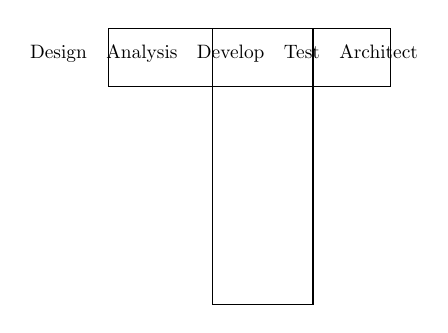
\begin{tikzpicture}[x=0.75pt,y=0.75pt, yscale=-0.7,xscale=0.7]
%Shape: Rectangle [id:dp793644495324062] 
\draw   (318,25.2) -- (387,25.2) -- (387,215.2) -- (318,215.2) -- cycle ;
%Shape: Rectangle [id:dp3939879341512962] 
\draw   (246.5,25) -- (440.5,25) -- (440.5,65.2) -- (246.5,65.2) -- cycle ;
% Text Node
\draw (191,35) node [anchor=north west][inner sep=0.75pt, yscale=0.7,xscale=0.7]   [align=left] {Design \ \ Analysis \ \ Develop \ \ Test \ \ Architect};
\end{tikzpicture}
  \caption{T-shaped person}
\end{minipage}
\end{figure}
Having a broad set of skill enhance collaboration and allow for better feedback inside the team itself. The end goal of Scrum teams is to deliver products iteratively and incrementally, while maximizing opportunities for feedback.

\subsubsection{The product owner}
The Product Owner is responsible for maximizing the value of the product resulting from the work of the Development Teams. The task mainly focus on the ensuring clarity over what is required and what need to be done. This encompasses managing the Product Backlog (the concept will be later explained). The product owner decisions can be seen from the Backlog.\\
\subsubsection{The Development Team}
The Development Team consist of professionals who do the work of delivering a potentially releasable Increment of "Done" product at the end of each sprint. Only the members of the Development Team can deliver a product increment. \\
The Development Team need the following characteristics:
\begin{itemize}
    \item They are self-organizing. A potentially releasable functionality is chosen from the members, not even the Scrum Master can influence this choice. 
    \item Development Teams need to be cross-functional. 
    \item Accountability belongs to the Development Team as a whole. 
\end{itemize}
Development team size is small enough to remain nimble and large enough to complete work in the Sprint.
\subsubsection{The Scrum Master}
The Scrum Master is responsible for promoting and supporting Scrum. Scrum Masters do this by helping everyone understand Scrum theory, practices, rules and values. 
The Scrum Master need also to interface between the Scrum Team and those on the outside, his success is related to the success in the interactions, in order to maximize the value created by the Scum Team. The following interfaces roles are required to the Scrum Master:
\begin{itemize}
    \item Scrum Master to the Product Owner, ensuring that goals, scope and product domain are understood by the Product Owner and the Backlog resemble those objectives.
    \item Scrum Master to the Development Team, coaching team on self-organization and cross-functionality while ensuring that high quality products are outputted. 
    \item Scrum Master to the Organization, helping stakeholder understand the empirical product development and work, act as an intermediary for the communication from outside to the Scrum team. 
\end{itemize}

\subsection{Scrum Events}
Scrum is composed by a series of regularly planned meetings. All the events are time boxed events, such that they respect a maximum duration. A scheme of how the Scrum process run is reported in \ref{figscrum}.
\begin{figure}[H]
    \begin{center}
        \begin{tikzpicture}[scale=0.50,transform shape,, node distance=4cm,>=latex']
        \node [input, name=input] {};
        \node [sum, right of=input] (sum) {};
        \node [block, right of=sum] (Prod_Backlog) {$Product\;Backlog$};
        \node [block, right of=Prod_Backlog] (Sprint_Plan) {$Sprint\;Planning$};
        \node [block, right of=Sprint_Plan] (Sprint_Backlog) {$Sprint\;Backlog$};
        \node [block1, right of=Sprint_Backlog] (Sprint_scrum) {$Scrum\;Sprint$};
        \node [block, below of=Sprint_scrum] (daily) {$Daily\;Scrum$};
        \node [block, above of=Sprint_scrum] (Retrospective) {$Retrospective$};
        \node [block, right of=Sprint_scrum] (Sprint_rev) {$Sprint\;Review$};
        \node [output, right of=Sprint_rev] (output) {};
        \draw [draw,->] (input) -- node [above left] {$Requirements$} (sum);
        \draw [->] (sum) -- node {} (Prod_Backlog);
        \draw [->] (Prod_Backlog) -- node {} (Sprint_Plan);
        \draw [->] (Sprint_Plan) -- node {} (Sprint_Backlog);
        \draw [->] (Sprint_Backlog) -- node {} (Sprint_scrum);
        \draw [->] (Sprint_scrum) -- node {} (Sprint_rev);
        \draw (Sprint_rev)--++(90:1) coordinate (A)--++(90:3) ;
        \draw [->] (Retrospective) -| node [above, pos=0.79] {} (sum) ;
        \draw [<->] (Sprint_scrum) -- node [] {} (daily) ;
        \draw [->] (Sprint_rev) -- node [name=y, above] {$Product\;Delivery$}(output);
        \draw [->] (y) |- node [above, pos=0.79] {} (Retrospective) ;
        \draw[->] (y)--++(-90:1) coordinate (A)--++(-90:4.5) coordinate (B)-|(sum);
        \end{tikzpicture}
    \end{center}
    \caption{Scrum process}\label{figscrum}
\end{figure}
In the scheme the five Scrum events can be found:
\begin{itemize}
    \item Sprint planning 
    \item Scrum Sprint
    \item Sprint review 
    \item Daily Scrum 
    \item Sprint Retrospective
\end{itemize}
\subsubsection{The sprint}
The heart of the Scrum is the Sprint, a time-box of one month or less in which a "Done", usable and potentially releasable product increment is created. In general sprints are consequential to each other, so as soon as a sprint ends a new one stars. \\
Sprint can be thought as a project with a short horizon. As projects also sprint need to accomplish something. Each sprint therefor has a goal of what is to be build, a design and a flexible pane that will guide the development team.\\
The time limitation of the sprint avoids the risk of changes in what is being build. With long sprint complexity of the goal may arise, and with that also the risk of failing. Having a sprint with a maximum length of a month ensures that at least monthly an adaptation and inspection of the progress toward a goal is implemented. 
\subsubsection{Sprint Planning}
The work to be performed in the Sprint is planned in this event. The collaborative team create a plan to work on for the next sprint. \\
Sprint planning is also a time-boxed event, which duration may vary in regard to the duration of the sprint.\\
In this event the development team forecast the functionality that will be developed during the Sprint. The product Owner discuss the goal that the sprint should achieve. The team than decide which of the items present in the product backlog integrate in the sprint and define a spring goal to go along with it.\\
The inputs of this meeting are the Product Backlog and the latest increment. The teams select the product backlog items and defines a goal. With the performance during last increment the team also define the load of work it needs to take on for the next sprint. All of this together compose the so called \textit{Sprint Backlog}.\\
The Sprint goal is an objective set for the Sprint that can be met thought the implementation of the Sprint Backlog. 
\subsubsection{Daily Scrum}
Daily scrum is a 15-minute time-boxed event for the development team, the meeting is held every day.\\
In the event the development team inspect the progress towards the Sprint goal and how progress is trending toward completing the Sprint Backlog. The Daily Scrum enhance the communication between team members, therefor the structure of the meeting is based on the question "what work I am currently doing in order to full fill the Sprint Goal?".
\subsubsection{Sprint review}
A Sprint Review is held at the end of a Sprint to inspect the increment and adapt the Product backlog. During this event the Scrum team and the stakeholder discuss the output of the Sprint. The meeting should sparkle feedback from the last released increment, in order to improve the Backlog.\\
The result of this meeting is a revised product Backlog that defines the probable Product Backlog items for the next sprint.
\subsubsection{Sprint retrospective}
This event is an opportunity for the Scrum Team to inspect itself and create a plan for improvements to be enhanced during the next Sprint. The purpose of the Sprint Retrospective is to:
\begin{itemize}
    \item Inspect how the communication between the team worked.
    \item Identify potential improvements.
    \item Think on how improvements can be implemented
\end{itemize}
The main focus of the team is to improve the work process. The underlined improvements should be implemented in the next sprint. This allow the team to mold the Scrum process on its need, still maintaining a structured approach. 
\subsection{Scrum Artifacts}
Scrum relies on transparency, therefore Scrum artifacts are designed to maximize transparency. This allow everyone to have a clear understanding of the state of the process.
Artifacts are composed both by tools but also team defined concepts such as the "Definition of Done". The Artifacts of Scrum are the following:
\begin{itemize}
    \item Product Backlog;
    \item Sprint Backlog;
    \item Definition of Done. 
\end{itemize}
\subsubsection{Product Backlog}
The product Backlog list all the requirements that the final product need. Obviously the initial lay out of the Backlog is not the complete one. At the beginning this Artifact list only the available requirements. Then, with the product evolving through the development process, the Backlog gets updated with new requirements.\\

The fact that the Backlog continuously changes reflect one important Agile principle, the one of accepting new requirements throughout the whole development process. It´s in the Scrum nature to welcome changes during the whole development.\\

The backlog not only gets updated with new requirements but also "refined". The act of adding details, estimating and ordering a Product Backlog is called "Refinement". With this process items of the Backlog are reviewed and revised. The ordering is done in such a way that the highly ordered product items are usually cleaner and more detailed that the lowered ordered ones. High Backlog items are "more" ready to be inserted in the Sprint, as the presence of more detailing reflects the fact that the team understand what and how the item can become part of the product. \\

Another important usage of the Product Backlog is related to monitoring the progress towards goals. Via the Backlog the product owner can easily tack the total work remaining to complete all the items, and therefor complete the product. 
\subsubsection{Sprint Backlog}
The Sprint Backlog is the set of Product Backlog items selected for a certain Sprint, plus a plan for delivering the product increment and therefor full fill the sprint goal.\\
Via the Sprint Backlog the team has a shared visualization of what is necessary to complete the Sprint Goal.\\
To ensure continuous improvement, the Sprint Backlog need to include at least a major Backlog items, that really add something conspicuous to the final product. This allow a stronger feedback at the end of the Sprint, which is fundamental to the Scrum process. 
\subsubsection{Increment}
The Increment is the sum of all the Product Backlog items completed during the Sprint. The increment sums up to all the previously released one, composing the Product.\\
An increment need to full fill the team definition of "Done".
\subsubsection{Definition of "Done"}
A Sprint Backlog items can be defined as "Done" only if it meet the team definition of "Done". This definition is team-based, different teams can have different definition. The sum of all the "Done" items create a "Done" increment. This increment need to be usable. It´s important that the definition is chosen internally by the team, obviously the definition can vary slightly during the development, even if some basic rules need to be applied.
\subsection{Example of a Scrum application}
Having described completely the theory behind the approach, the feeling is the one I personally had the first time learning about Scrum. The method have potentials, but the application does not seem that revolutionary. In this sense, I provide here an example which explain how a product is developed using Scrum. This should give a general idea over the method, helping to understand how a possible application can take place. In the \ref{fig:scrumprddev} the full development of a Product using Scrum is reported.
\begin{figure}[htp]
    \centering
    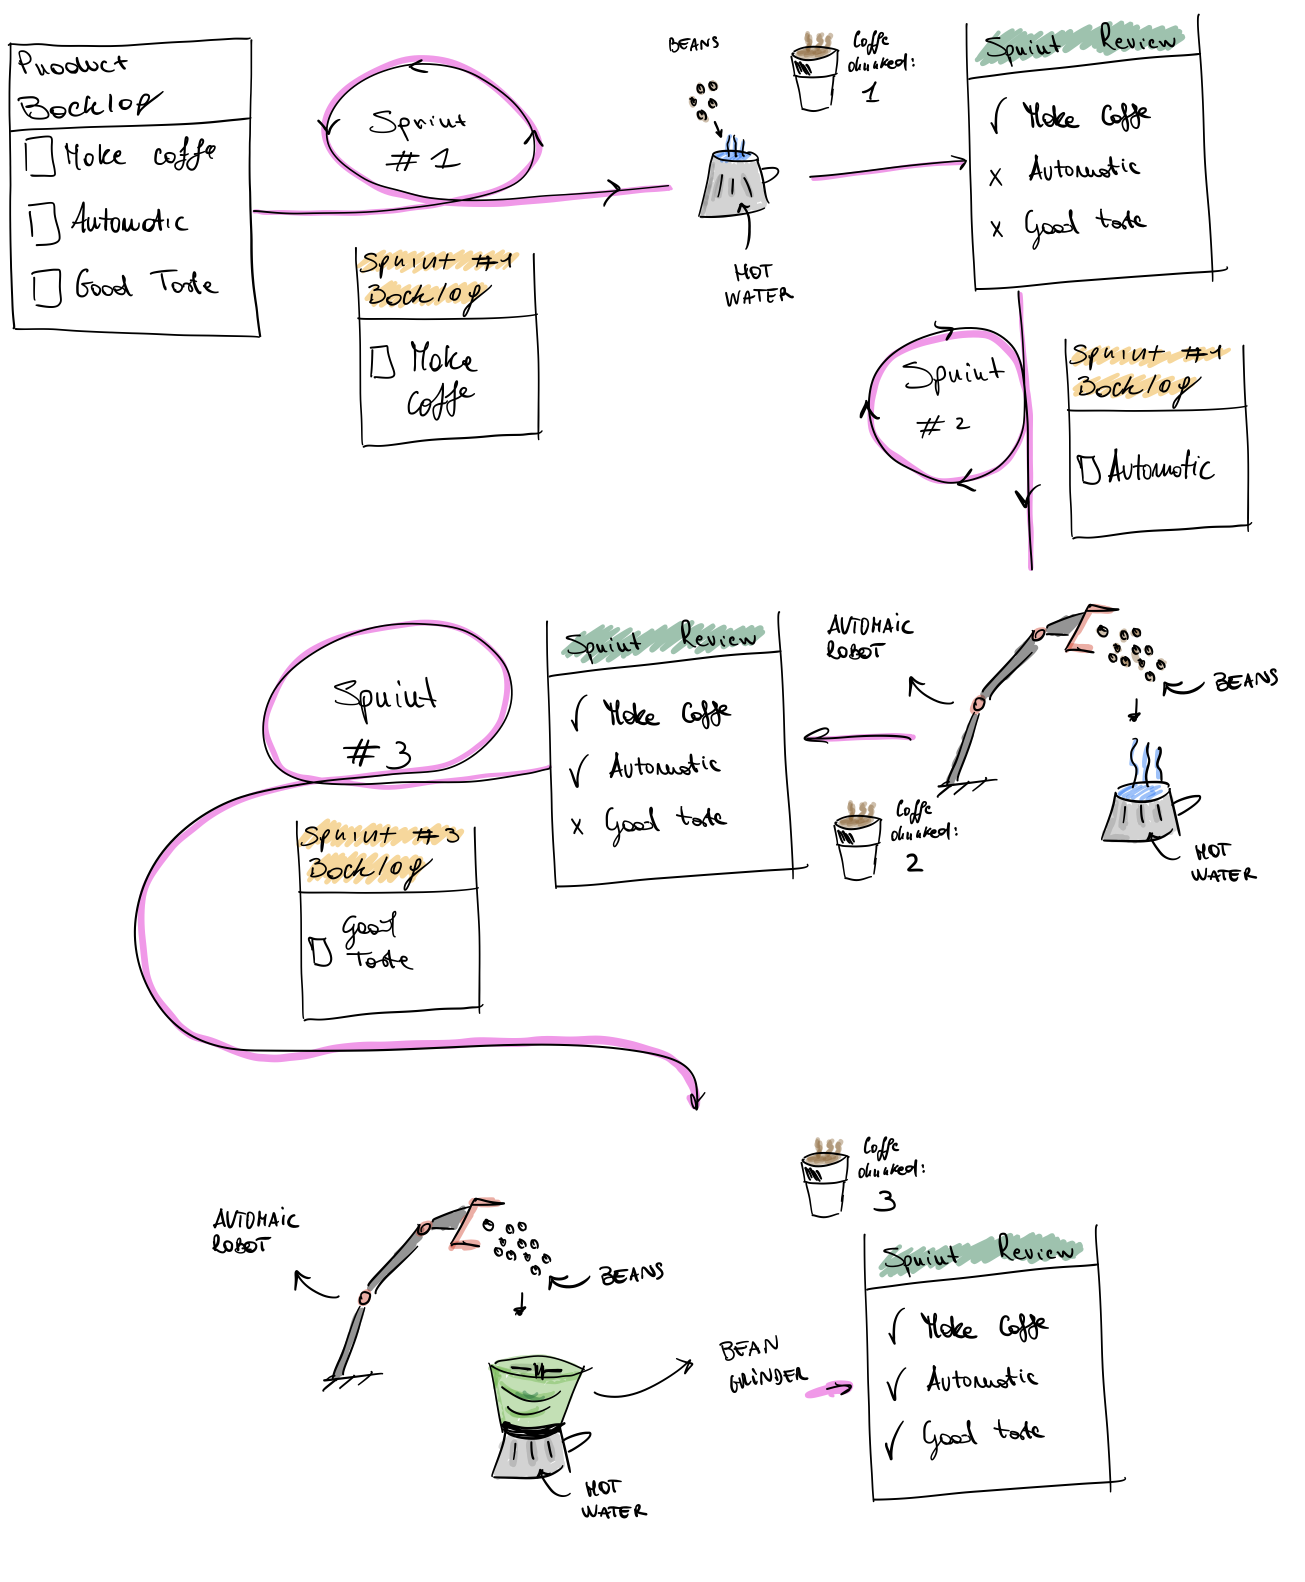
\includegraphics[width=\linewidth]{images_folder/scrum.png}
    \caption{Scrum product development}
    \label{fig:scrumprddev}
\end{figure}
At the beginning (top left corner) the process start with the definition of the requirements, which compose the Product Backlog. For the sake of simplicity we consider to have the full set of requirements at the beginning of the process. The team, as first task, also defines its own definition of "Done". They,  the team, opted to define "Done" increment as one completely full filling a certain requirement. This indeed comprehend not only designing, but also testing and integrating, having therefor a working product at the end of each sprint.\\
Starting the first sprint, considering a capacity of 1 Backlog item per sprint the team decides to implement the task "\textit{make coffee}". This task is the one which brings the highest value to the product at the end of the sprint. The "Sprint \#1 Backlog" is therefor composed by only this task.\\
At the end of the first sprint the team presents to the Business Owner and to the Stakeholders the "Done" increment, in this case a mug, containing hot water in which pour the coffee beans. The team has the opportunity to check its progress and get a direct feedback from the stakeholders.\\ Here the team has already drank a cup of Coffee. This is going to be important later.\\ The scrum continues until the final sprint, in which the team output a complete automatic coffee machine. Prior to the release on the market the team has drank 3 total Coffee during the development process. At the end the Backlog is empty, since all the tasks have been completed. 
\subsection{Waterfall vs Scrum}
In order to completely understand the advantages of Scrum in regard to classic techniques, the methodology is compared with the classic approach of Waterfall development. 
\begin{figure}[H]
\centering
    \begin{tikzpicture}[>=stealth]
     \node[phase]                       (requirements)  {\small Requirements};
      \node[phase,previous=requirements] (design)       {\small Design};
      \node[phase,previous=design]       (coding)       {\small Coding and\\unit test};
      \node[phase,previous=coding]       (integration)  {\small System\\integration};
      \node[phase,previous=integration]  (operation)    {\small Operation and\\maintenance};
      \connectow{requirements}{design};
      \connectow{design}{coding};
      \connectow{coding}{integration};
      \connectow{integration}{operation};
    \end{tikzpicture}
\caption{Waterfall model}
\end{figure}

Waterfall methods are still in great usage, the main feature is that the development is done step by step, flowing from a stage to the other. As \cite{Scrum} refers they based on a scheme where "each piece of the project cascade down to the next like a waterfall". The methodology lays out everything using the \textit{Gant charts}. One of the criticism that the authors of Scrum made is related exactly to those charts, that are as complex as wrong. Here is reported a development of a product similar to the one reported in \ref{figscrum} but using a waterfall approach.\\
\begin{figure}[H]
    \centering
    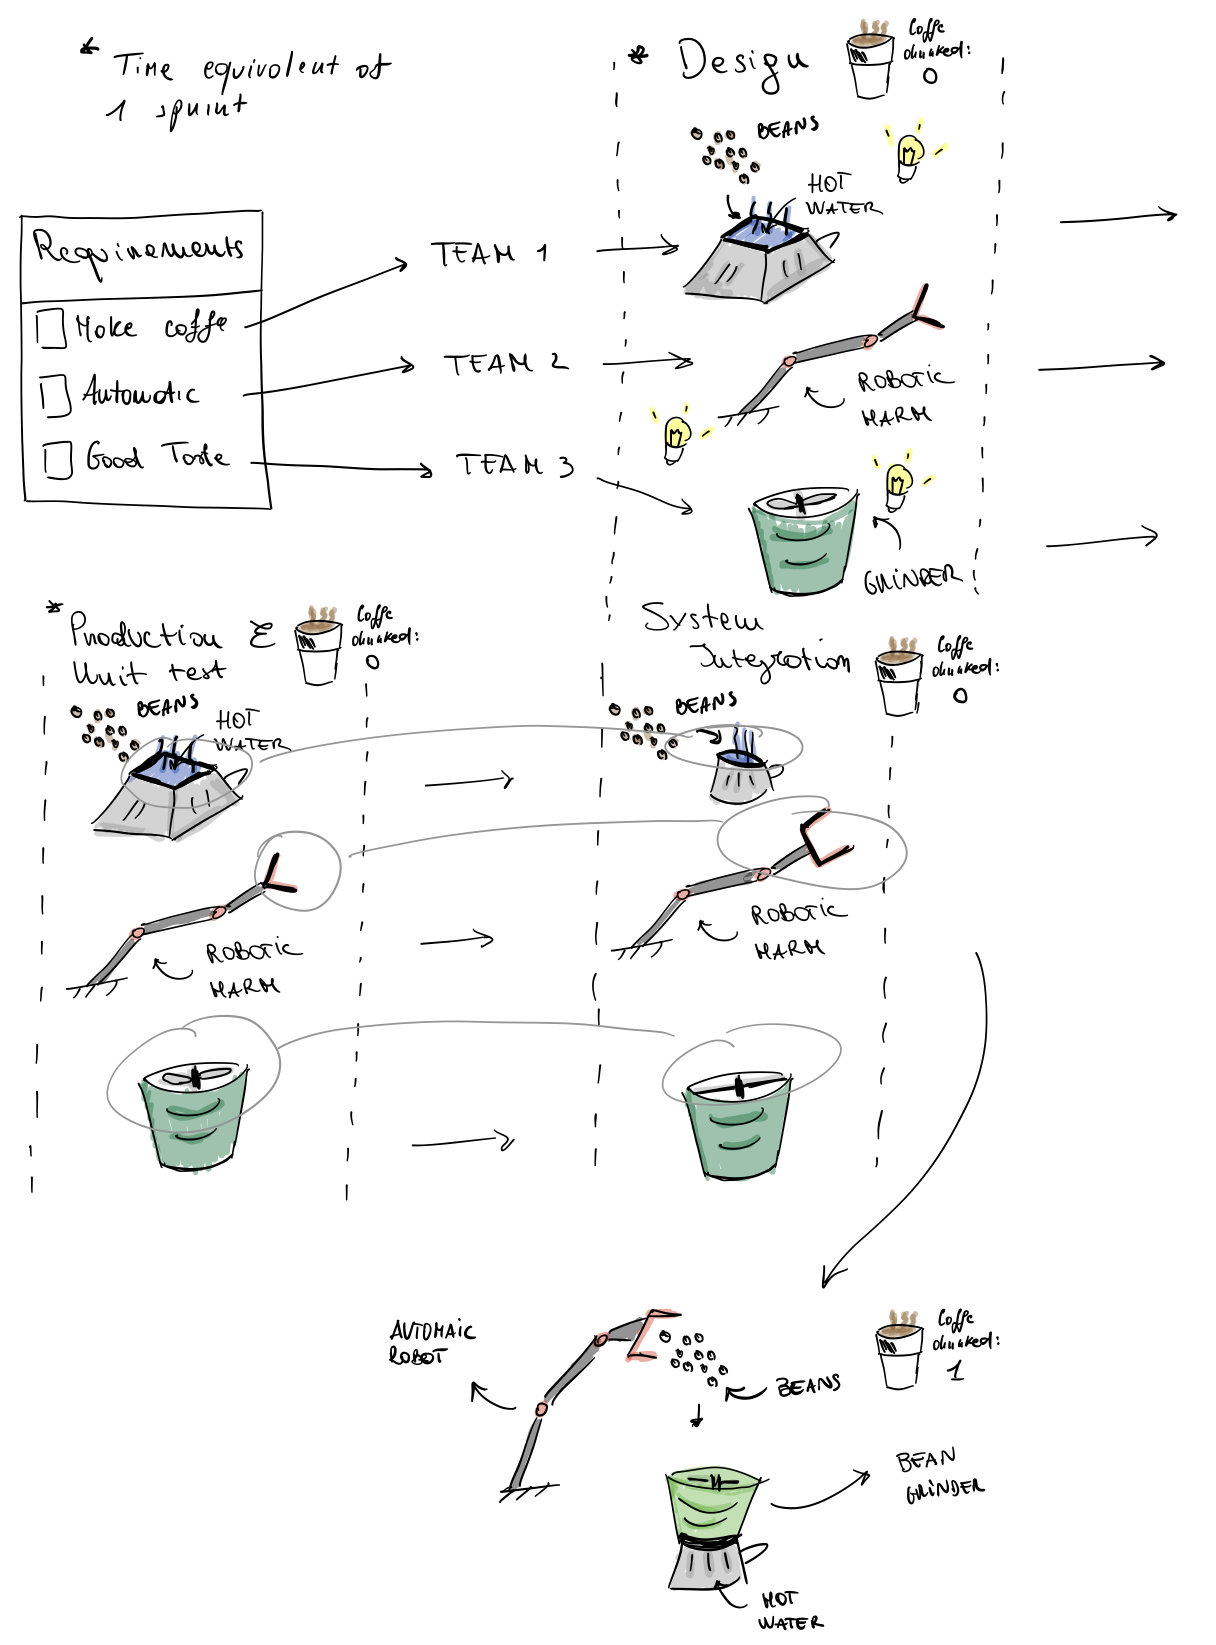
\includegraphics[width=\linewidth]{images_folder/waterfall.png}
    \caption{Waterfall product development}
    \label{fig:swaterrddev}
\end{figure}
The task is the same described in the Scrum process, the required product is an automatic coffee machine. The team, following the waterfall method splits in sub teams for the first step of components design. The outputs of what in a time manner could be compared to a Scrum Sprint are the ideas on how to full fill the requirements. The next step is the production and unit test of each components. Each team in the example produces and test the assigned components. The output of the second step in the process are the fully completed components. The last step is integration. The teams, integrate the components with the other developed by different groups. Obviously the process is not flawless, because the team only discover at this step how the others developed a certain requirements. At the end the team full fill all the requirements and release a product identical to the one developed following the Scrum methodology.\\ There are, indeed a lot of differences, which favor the Scrum approach.
\begin{itemize}
    \item During the whole development process the Waterfall approach has no direct feedback from the stakeholders, no coffee is drank by the team before the product is released. This mean that the first feedback arrives at the end of the development process where, recalling \ref{fig:agilevswaterfall} the cost for a adjustment is higher. 
    \item The team has no way of predicting the correct time that it will take to deliver a product. This can be really vary based on the integration between the different parts designed by the teams. A no fit in this situation would set the team back just for one of the components. 
    \item Scrum offers the opportunity to prioritize requirements. The requirement who bring the most value to the product need to be the first one implemented. In this case making coffee. This allow for not only direct feedback on key product features, but also allow to stop in case a product is defined as completed, just by having part of the overall desired features. 
\end{itemize}
\cleardoublepage
\end{document}